\documentclass[12pt]{article}
\usepackage[a4paper, margin=1in]{geometry}
\usepackage{graphicx}
\usepackage{amsmath}
\usepackage{hyperref}
\usepackage{bookmark} % Add bookmark package to handle outline changes
\usepackage{titlesec}
\usepackage{setspace}
\usepackage{enumitem}
\usepackage{natbib}
\usepackage{tikz}
\usepackage{amssymb}
\usepackage{float}
\usepackage{booktabs}
\usepackage{todonotes}
\usepackage{amsthm}

% Define the proposition environment
\newtheorem{proposition}{Proposition}
\usetikzlibrary{trees}
\titleformat{\section}{\normalfont\Large\bfseries}{\thesection.}{1em}{}
\titleformat{\subsection}{\normalfont\large\bfseries}{\thesubsection.}{1em}{}

\title{Network Games and Agricultural Collectivization in China}
\author{Xinkai Xu, Liming Lin, Zihao Liu}
\date{\today}

\begin{document}

\maketitle
\onehalfspacing

\begin{abstract}
  This project uses the framework of network games to analyze agent behavior during Chinese agricultural collectivization in the 1950s–60s. While prior studies explain the crisis through free-riding \citep{chinnDiligenceLazinessChinese1980, lin1990collectivization}, this paper focuses on peer effects. Starting from a small reciprocal team model with complete information, we extend the framework to larger inter-connected networks and incorporate signaling games to investigate the effects of government propaganda. Numerical simulations show that as networks grow and information becomes incomplete and diffuse, equilibrium effort levels decline, which potentially explain the decrease in productivity when small reciprocal groups were expanded into large People's commune. We also examine the role of government propaganda, finding that positive propaganda increase agents’ efforts, while negative propaganda reduce them.
\end{abstract}

\section{Introduction}
China's large population and limited arable land made agricultural collectivization an appealing strategy to achieve economies of scale. However, it also introduced classic free rider problems. Previous research has primarily attributed the decline in individual effort during the transition from small reciprocal groups to People's Communes to these free rider issues.\citep{chinnDiligenceLazinessChinese1980,lin1990collectivization}

In this paper, we offer a new perspective by emphasizing the role of peer effects. While collective farming can generate informal incentives through peer monitoring and social norms, these effects depend heavily on the structure of the network and the availability of information. In the small reciprocal groups period, individuals were closely connected and had full knowledge of one another's behavior, which fostered strong peer effects. We capture this setting by modeling effort choices in a complete information game on a fully connected network.

However, under the People's Commune system, social ties became more diffuse and individuals were less familiar with one another. This weakened the peer effect, largely due to incomplete information. To reflect this, we build a new game-theoretic model on a bridge network, where the complementarity of effort between individuals—represented by a parameter $\beta$ which represents the incomplete information setting. This allows us to analyze how incomplete information about others' behavior contributed to the decline in effort.

Moreover, we incorporate government propaganda into the model, as the state actively attempted to shape farmer behavior during the People's Commune era. Two main forms of propaganda were used: one celebrated model workers (labor heroes) to inspire others, while the other criticized so-called “lazy” or “backward” individuals. We model these as two types of signals that influence individuals' beliefs about the complementarity parameter $\beta$. By integrating these signals into an incomplete information network game, we study how different propaganda strategies affected individual effort under the institutional conditions of the People's Commune.

We can also empirically test some implications of the model. First, we can examine whether regions with stronger collectivist values had higher reported output during the People's Commune period, which would reflect the influence of ppp on outcomes. Second, we can investigate whether regions with more model workers (labor heroes) had higher output, which would reflect the impact of positive propaganda on outcomes.

\section{Base Model: The Small Network within a Commune}
In the early stages of rural collectivization, agricultural production was organized through mutual-aid teams, typically consisting of a handful of neighboring households. These small groups were built upon existing social ties, such as kinship, proximity, and shared village identity. Within such closely-knit settings, individuals were able to observe each other’s behavior directly, fostering a high degree of mutual monitoring and reciprocal expectations. This justifies the modeling assumption of complete information, where each agent has accurate knowledge of their peers’ effort levels. In this environment, peer effects are strong, and cooperative behavior is sustained by informal social norms and reputational incentives.\\

Let $I = \{1, 2, \dots, n\}$ denote the set of players, $n > 1$, connected by a network $G$. We use matrix $G$ to track the connections in this network. We define $g_{ij} = 1=g_{ji}$ if $i$ and $j$ are linked to each other, and $g_{ij} = 0$ otherwise.  We also set $g_{ii} = 0$. The neighborhood of the individual $i$ is the set given by $ N_i := \{j \ne i \mid g_{ij} = 1\}$. Therefore, $|N_i|$, the cardinality, which is $\sum_j^n g_{ij}$, is called the \textbf{degree} of $i$.\\

We use the following quadratic utility function to capture the \emph{strategy complementarity}:
\[
U_i(x_i, x_{-i}, G_i) = \alpha x_i - \frac{1}{2} x_i^2 + \beta \sum_j g_{ij}x_i  x_j,
\]

where $\alpha$ is the marginal return to effort $x_i$, and $\beta$ is the strength of strategic interactions.

We assume $\beta > 0$, so that we have
\[
\frac{\partial^2 U_i(x_i, x_{-i}, G_i)}{\partial x_i \partial x_j} = \beta g_{ij} > 0,
\]
which reflects strategic complementarity in efforts.

In small groups with $n$ players in a network, people know each other well, and it is reasonable to assume network $G$ is a \textbf{complete network} and players have full information.

\begin{figure}[H]
  \centering
  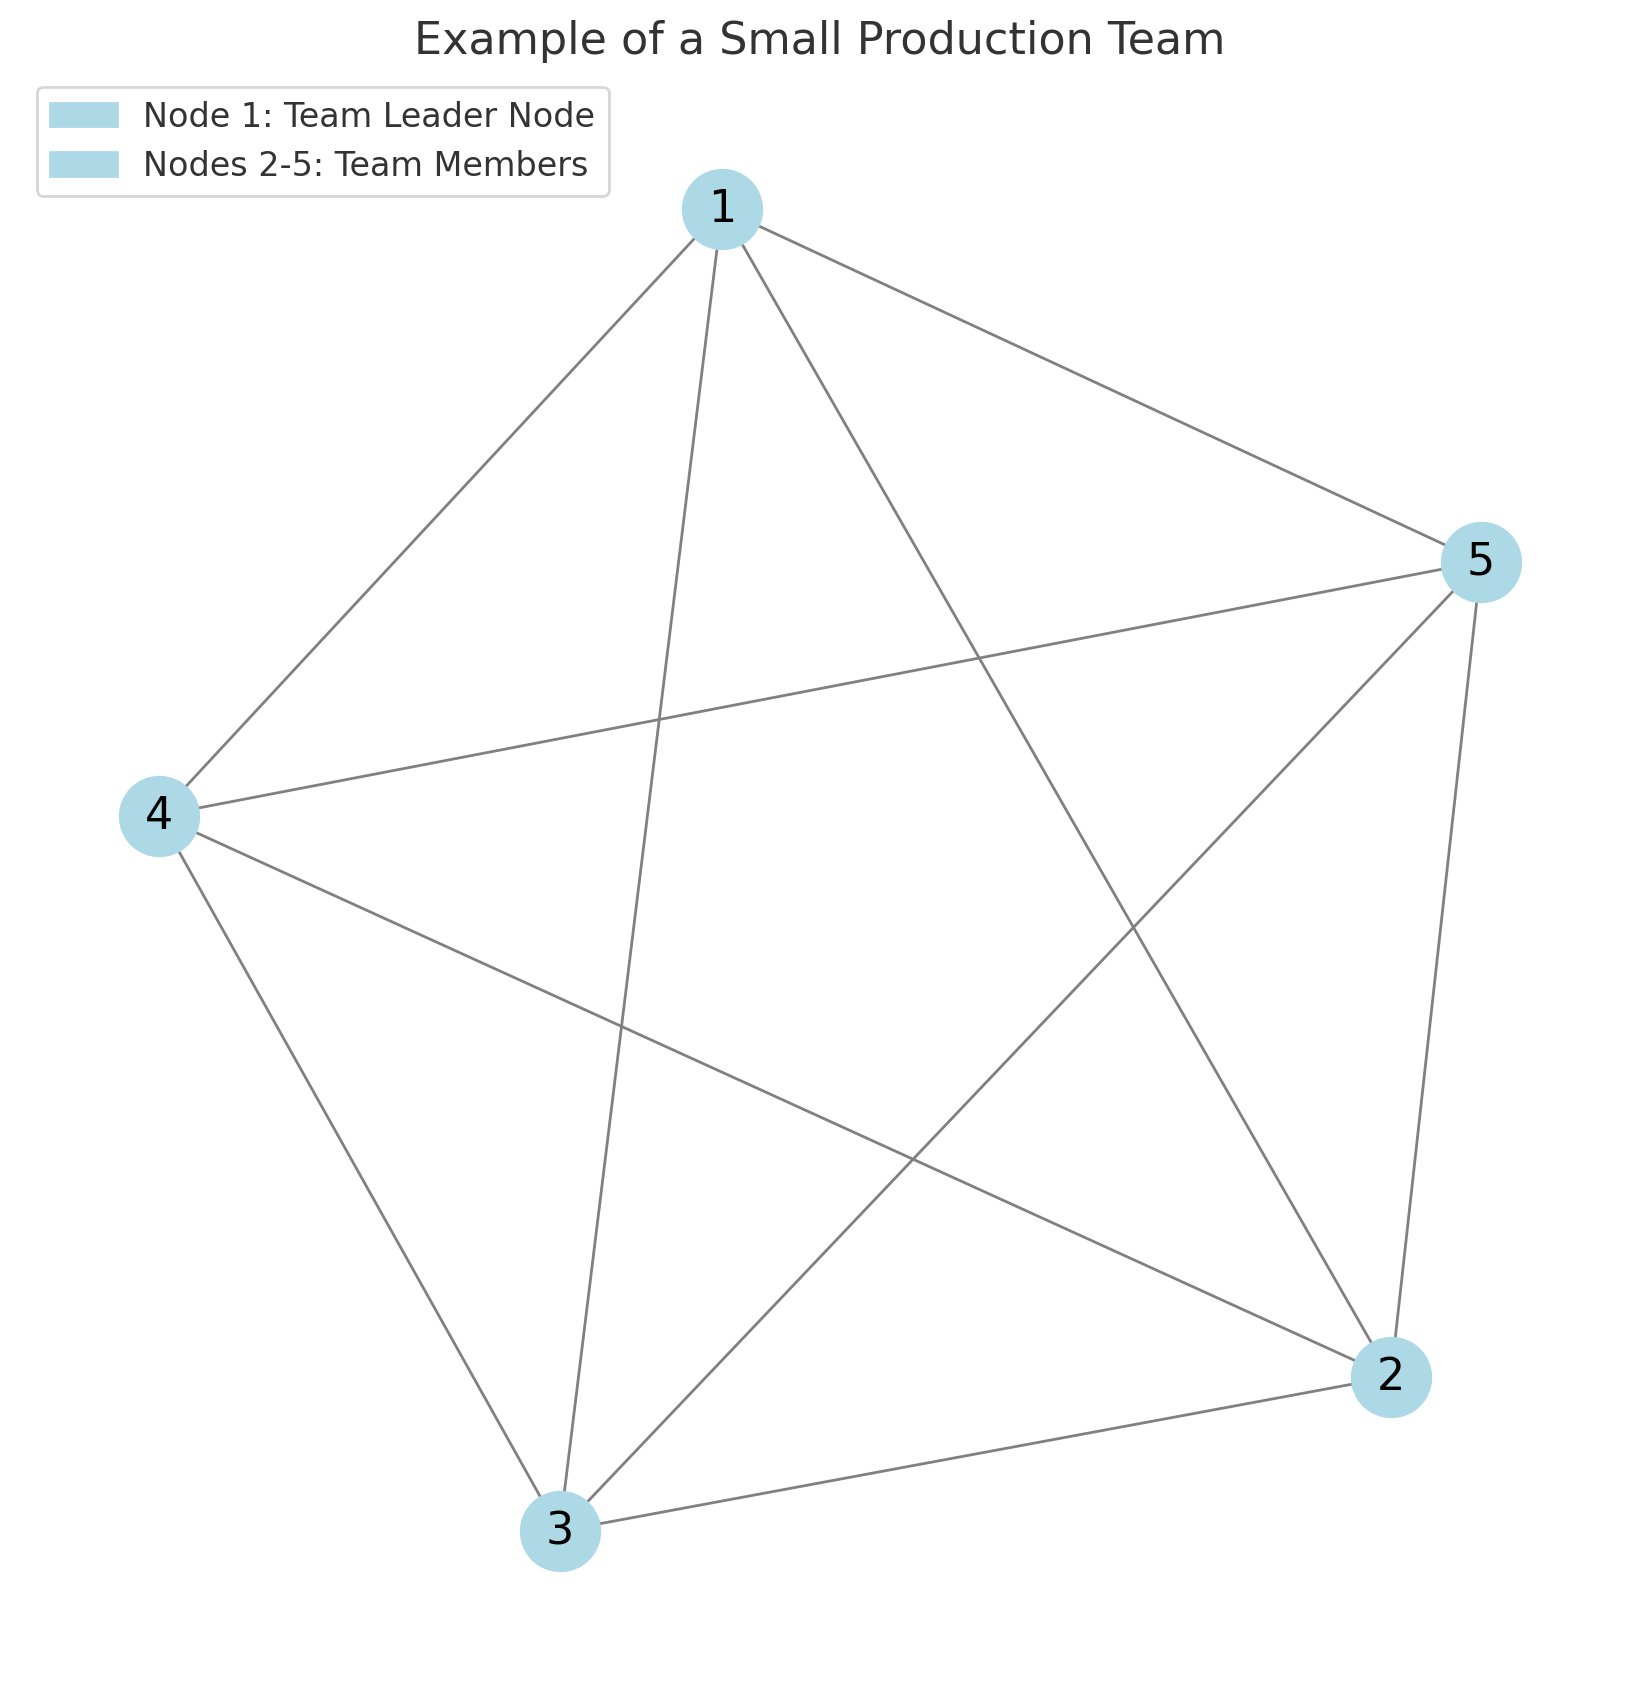
\includegraphics[height=0.6\textwidth]{small network1.png}
  \caption{Example of a Small Production Team}
  \label{fig:small-team}
\end{figure}

In equilibrium, each agent maximizes their utility. By the FOC, we get:
\[
x_i^* = \alpha + \beta \sum_j g_{ij} x_j. \tag{2}
\]

Since $G$ is a complete network, everyone has the same degree. We assume total effort is  
\[
\bar{x} = \sum_i x_i,
\]
and so:
\[
x_i^* = \alpha + \beta (\bar{x}-x_i^*) = \alpha + \beta(n x_i^*-x_i^*).
\]
Rearranging gives:
 we get:
\[
x_i^* = \frac{\alpha}{\beta+1-n \beta}.
\]
In order to compare the equilibrium efforts in this small network setup with the large network modesl we will have later, we calculate here using $n=5$ and $\beta=0.06$ to get $x^*_{small} \approx 1.3157$.
\section{Large Networks}
\subsection{Large Network with Without Signaling}
Now we move to the large network setting where there are multiple small groups. As the collectivization campaign intensified, the state consolidated small reciprocal groups into much larger units known as People’s commune. These communes often encompassed multiple villages and hundreds or even thousands of households, significantly diluting the social connections that underpinned smaller collectives.\\
In this setting, most individuals no longer had personal knowledge of their fellow members’ actions or intentions. The social distance and anonymity introduced by the larger and sparser network structure resulted in a breakdown of direct peer monitoring and communicating. \\
To reflect this, we model large networks under the assumption of incomplete information: agents no longer observe others' effort directly and must form expectations based on priors. Consequently, peer effects weaken, and cooperative norms erode as uncertainty and distrust proliferate. And in each small complete network, there is one node that represents the leader of the small group. Between the small groups, there are indirect connections among the small group leaders through a central node the represents higher level government.\\
By this construction, we have three types of players with different degrees.  
We assume $N = nk + 1$, where $n$ is the number of players in a small group, $k$ is the number of small groups.

\begin{itemize}
    \item Type 1: $(n-1)$ degrees (group members)
    \item Type 2: $k$ degrees (higher level leaders)
    \item Type 3: $n$ degrees (small group leaders)
\end{itemize}

\begin{figure}[H]
  \centering
  \includegraphics[width=0.7\textwidth]{large network1.png}
  \caption{Example of a Large Network}
  \label{fig:large-network}
\end{figure}

In our models, we denote $\beta$ as incomplete information to capture the feature that in large groups, an agent does not know their neighbors' neighborhoods well, where $\beta$ takes two possible values: $\beta = \{\beta_l,\beta_h\}$ where $\beta_l < \beta_h$. 

All agents share a common prior:

\[
\mathbb{P}(\beta = \beta_h) = p, \quad \mathbb{P}(\beta = \beta_l) = 1-p
\]

In addition, we assume there is no communication between players, and the network does not affect the value of $p$.

Then:

\[
\mathbb{E}[u_i] = \alpha x_i - \frac{1}{2}x_i^2 + \mathbb{E}[\beta] \sum_{j=1}^{n} g_{ij} x_i x_j
\]

where:

\[
\mathbb{E}[\beta] = p \beta_h + (1-p) \beta_l
\]

The first order condition with respect to $x_i$ gives:

\[
\frac{\partial \mathbb{E}[u_i]}{\partial x_i}= \alpha - x_i + \mathbb{E}[\beta] - \sum_{j} g_{ij} x_j = 0
\]

\vspace{1em}

Rearranging gives:

\[
x_i^* = \alpha + \mathbb{E}[\beta] \sum_{j=1}^{n} g_{ij} x_j
\]

\vspace{1em}

Factoring out $\alpha$ gives:

\[
x^* = \alpha (I_n - \mathbb{E}[\beta] G)^{-1} \mathbf{1}
\]

where $I_n$ is the $n \times n$ identity matrix, $G$ is the network matrix for our model and $1$ is a matrix of ones.

\vspace{1em}

In order to find a unique nash equilibrium, we need to make sure that the matrix $(I_n - \mathbb{E}[\beta] G)$ is invertible. This is equivalent to ensuring that $\mathbb{E}[\beta]$ is less than the largest eigenvalue of $G$.

\[
\mathbb{E}[\beta] < \frac{1}{\lambda_{\text{max}}(G)}
\]

Wihtin the formula for equilibrium efforts, we also have the formula for Bonacich centrality which is given by:
\[
b(\beta, G) = \sum_{k=0}^{\infty} \beta^k G^k I_n = (I_n - \beta G)^{-1} l_n,
\]
\vspace{1em}

Then we can rewrite the equilibrium effort as:
\[
x_i^* = \alpha b_i(\mathbb{E}[\beta], G) \mathbf{1}
\]

in which $i$ denotes $i$th agent.\\
\vspace{1em}
Given the structure of the network, here is the $G$ matrix that represents the connections between players:
\begin{figure}[H]
  \centering
  \includegraphics[width=0.7\textwidth]{Default_Large_Network_Labeled.png}
  \caption{Adjacency matrix $G$ for the default 16-player network}
  \label{fig:G-matrix}
\end{figure}
So the 1st, 9th, and 12th rows are the leaders of the small groups, while the 16th row (the last row) is the central node that connects all the small group leaders. The rest are the members in the small groups.\\
Then we calculate the eigenvalues of the $G$ matrix. (See in appendix) The largest eigenvalue is $\lambda_{\text{max}}(G)  \approx 4.1622$ and thus the upperbound for $E[\beta] = \frac{1}{\lambda_{max}(G)} \approx 0.24$.\\
\subsubsection*{Numerical Simulations}
Again, for the sake of comparison among models, we assume that $\beta_h=0.06$ and $\beta_l=0.03$ and $p=0.5$ for now. Note that $\beta_h$ takes the same value as $\beta$ in the small reciprocal group, which represents the value in complete network. With incomplete information, there are some agents holds belief $\beta_l$ here. The resulting $\mathbb{E}[\beta]=0.045$ which conforms to the upperbound we just calculated. We leave $\alpha$ as a undetemined parameter for now.\\
\begin{table}[H]
  \centering
  \begin{tabular}{lcc}
  \toprule
  \textbf{Player Type}  & \textbf{\( x^* \) when \( E[\beta] = 0.045 \)} \\
  \midrule
  Small Group Leader        & 1.27 \\
  Small Group Member        & 1.22 \\
  Central Leader (Player 16)  & 1.17 \\
  \bottomrule
  \end{tabular}
  \caption{Equilibrium actions \( x^* \) in large network with incomplete information and without signaling}
  \label{tab:xstar-beta}
  \end{table}
In contrast to $x^*_{small}$ we had previously, $x^*_i$ for all types of players have smaller equilibrium efforts.\\
\begin{proposition}
  The equilibrium efforts decrease as small reciprocal groups are expanded into large People's Communes, such that:
  \[
  x^*_i < x^*_{\text{small}} \quad \text{for all } i
  \]
  \end{proposition}
  Which can be attributed to the fact that due to incomplete information, agents receive $E[\beta]$ less than the $\beta$ in the small reciprocal group that is a complete network. This leads to a decrease in the equilibrium efforts.\\
Besides, the results also show that group leaders have the highest equilibrium, following by group members and central leader, corresponding to the fact that the group leaders have the highest numbers of nodes connected, while the central leader has the least.\\
\subsubsection*{The Effects of $p$ on Equilibrium Efforts}
Additionally, we want to investigate how the equilibrium effort \( x^* \) changes with the value of \( p \) which is the probability of being a high type player. Here we return to the original equation for $E[\beta]$ which equals $p\beta_h+(1-p)\beta_l$. We assume $\beta_l=0.03$ and $\beta_h=0.06$. (So the $p=0.5$ case will have the same $E[\beta]$ as above.)  Again, doing differentiation is complicated so we plug in several possible values for $p \in [0,1]$\\
\begin{table}[H]
  \centering
  \begin{tabular}{lccc}
  \toprule
  \textbf{Player Type} & \textbf{\( x^* \) at \( p = 0.1 \)} & \textbf{\( x^* \) at \( p = 0.5 \)} & \textbf{\( x^* \) at \( p = 0.9 \)} \\
  \midrule
  Small Group Leader        & 1.19 & 1.27 & 1.37 \\
  Small Group Member        & 1.15 & 1.22 & 1.30 \\
  Central Government (Player 16) & 1.12 & 1.17 & 1.23 \\
  \bottomrule
  \end{tabular}
  \caption{Equilibrium actions \( x^* \) as a function of \( p = \mathbb{P}(\beta = \beta_h) \)}
  \label{tab:xstar-vs-p}
  \end{table}
The table above shows that the equilibrium effort \( x^* \) is increasing in \( p \) and thus $\mathbb{E}[\beta]$ which is aligned with the strategic complementarity. In other words, as people believe that there are higher level of strategic complementarity, they are more likely to exert higher efforts.\\ \textbf{Potential Empirical Test 1} In reality, we expect that $p$ may be increased with local collectivism culture: as people more likely to believe that their peers will hard, they will increase their own efforts. We can use survey data to measure the level of collectivist culture across regions and draw on grain output data from county-level statistical yearbooks to examine the impact of collectivist culture on production.\\
\subsection{Large Network with Signaling}
During the Chinese agricultural collectivization campaign of the 1950s and 1960s, the government relied heavily on propaganda to shape individual behavior within collective farming units. Positive propaganda was used to promote socialist ideals and incentivize effort, such as by publicly rewarding teams or individuals that worked hard. At the same time, negative propaganda was deployed to criticize or shame those perceived as lazy or noncompliant, often through public denunciations or political labeling. These communication strategies served not only to align individual incentives with state goals but also to influence beliefs and behavior. As a result, we introduce two types of signals to represent the government's propaganda and analyze their effects on agents' equilibrium efforts.

\subsection*{Model Setup}
To represent the set up described above, we now turn to \textbf{a large network model under incomplete information but with signaling}.

There are $M \gg n$ players now and we assume that $\beta$ can only take two values, $\beta_L$ or $\beta_H$.  
All individuals share a common prior:
\[
\Pr(\beta = \beta_H) = p, \quad p \in (0,1)
\]

Individuals receive two signals which are not always correct.  
We define:
\[
\Pr(s_i = h \mid \beta = \beta_h) = q = \quad \Pr(s_i = l \mid \beta = \beta_l) 
\]
where $s_i = h$ and $s_i = l$ denote the event that agent $i$ get to know the positive and negative propaganda. And we assume that $q \geq 0.5$ to reflect the accuracy of the propaganda signals sent by the government.\\

The idea is that a large network is composed of several small complete networks.  
And in each small complete network, there is one person who connects with leaders of the large group.

There are three types of players with different degrees.  
We assume $N = nk + 1$, where $n$ is the number of players in a small group, $k$ is the number of small groups.

\begin{itemize}
    \item Type 1: $(n-1)$ degrees (internal to small group)
    \item Type 2: $k$ degrees (one connection to each small group leader)
    \item Type 3: $n$ degrees (small group leader)
\end{itemize}

The utility function is the same for three types of players, given by:

\[
u_i(x_i, x_{-i}) = \alpha_i x_i - \frac{1}{2}x_i^2 + \left( \sum_j g_{ij} x_j x_i \right)
\]

We define:
\[
b(\beta, G) = \sum_{k=0}^{\infty} \beta^k G^k I_n = (I_n - \beta G)^{-1} l_n,
\]
where \( I_n \) is the identity matrix \( n \times n \) and \( l_n \) is the vector \( n \times 1 \) of 1.

When agent $i$ receives signal $s_i = l$, his utility function satisfies:


\[
\mathbb{E}[u_i \mid s_i = l] = \alpha \, \mathbb{E}[x_i \mid s_i = l]
-\frac{1}{2}\mathbb{E}[x_i^2|[s_i=l]]+ \sum_{j = 1}^n g_{ij} x_i\, \mathbb{E}[\beta x_j \mid s_i = l]
\]
\[
= \alpha \, x_i(l) - \frac{1}{2} x_i(l)^2 + \sum_{j=1}^{n} g_{ij} \, x_i(l) \, \mathbb{E}\left[ \beta \, x_j \mid s_j = l \right]
\]


Take the derivative with respect to $x_i$ gives us the first order condition:
\[
\alpha -x_i^*(l) +\sum_{j=1}^{n} g_{ij} \mathbb{E}[\beta x_j^* \mid s_i = l]=0
\]
Rearranging gives us:
\[
x^*_i(l) = \alpha_i(l) + \sum_j g_{ij} \mathbb{E}[\beta x_j \mid s_i = l]
\]



When agent $i$ receives signal $s_i =l$, for each possible $j$ we have:
\[
\mathbb{E}(\beta_j x_j \mid s_i = l) = \sum_{t=1}^{2} \\
\sum_{m=1}^{2} \beta_m x_j(t) P\left( \{\beta = \beta_m\} \cap \{s_j = t\} \mid s_i = l \right)
\]
\[
= \beta_{\max} \sum_{t=1}^{2} \left(\sum_{m=1}^2 P\left( \{\beta = \beta_m\} \cap \{s_j = t\} \mid s_i = l \right) \cdot \frac{\beta_m}{\beta_{\max}} \right)x_j(t)
\]

where $\beta_{max}$ =$\beta_h$ and $m\in[l,h]$

We define:

\[
P_{ll} = \sum_{m=1}^2 \mathbb{P}(\{\beta = \beta_m \}\cap \{s_j = t\} \mid s_i = l) \cdot \frac{\beta_m}{\beta_{\max}}
\]

 \  in our case.

$P_{ll}$ represents individual $i$ receives signal $l$ and $j$ receives signal $l$.

Therefore, we can rewrite the first order conditions as follows:

\[
\alpha - x_i ^*(l)+ \beta_{max}  \sum_{j=1}^{N}\ g_{ij} \sum_{t=1}^{2}p_{lt}*x_j(t)=0
\]
\[
\alpha - x_i ^*(h)+ \beta_{max}  \sum_{j=1}^{N}\ g_{ij} \sum_{t=1}^{2}p_{ht}*x_j(t)=0
\]

which can be characterized by:

\[
\begin{pmatrix}
x_l \\
x_h
\end{pmatrix}
= \left( I_{2n} - \beta_{max} (\Gamma\otimes G) \right)^{-1}
\begin{pmatrix}
\alpha_{1n} \\
\alpha_{1n}
\end{pmatrix}
\]

where $\Gamma$ is the information matrix, $G$ is the network matrix, $\otimes$ is the Kronecker product of $\Gamma$ and $G$.

$\Gamma$ is given by:

\[
\Gamma = 
\begin{pmatrix}
P_{ll} & P_{lh} \\
P_{hl} & P_{hh}
\end{pmatrix}
\]

Now we are going to calculate information matrix $\Gamma$.

We have:

\[
P(s_i = l) = P(s_i = l \mid \beta = \beta_l)P(\beta = \beta_l) + P(s_i = l \mid \beta = \beta_h) P(\beta = \beta_h)
\]
\[
=q(1-p)+(1-q)p
\]

We have:

\[
P(s_i = h) = P(s_i = h \mid \beta = \beta_h)P(\beta = \beta_h) + P(s_i = h \mid \beta = \beta_l) P(\beta = \beta_l)
\]


\[
= qp+(1-q)p
\]



\begin{align*}
&P(\{ \beta = \beta_l\} \cap \{ s_i= l \} \mid \{ s_i = l \}) \\
&= \frac{P(\{ s_j = l \} \cap \{ s_i = l \} \cap \{ \beta = \beta_l \})}{P(\{ s_i = l \})} \\
&= \frac{P(\{ s_j = l \} \mid \{ \beta = \beta_l \}) \, P(\{ s_i = l \} \mid \{ \beta = \beta_l \}) \, P(\{ \beta = \beta_l\})}{P(\{ s_i = l \})} \\
&= \frac{q^2(1-p)}{q(1-p)+ (1 - q)p}
\end{align*}

Similarly, we have
\[
P(\{\beta = \beta_h\} \cap \{s_j = h\} \mid s_i = l) = \frac{q(1-p)(1-q)}{q(1-p) + (1-q)p}
\]
and
\[
P(\{\beta = \beta_h\} \cap \{s_j = l\} \mid s_i = l) = \frac{p(1-q)^2}{q(1-p) + (1-q)p}
\]
as well as
\[
P(\{\beta = \beta_h\} \cap \{s_j = h\} \mid s_i = l) = \frac{(1-q)pq}{q(1-p) + (1-q)p}.
\]

Now, for \( p_{ll} \),
\begin{align*}
p_{ll} &= P\left( \{\beta = \beta_h\} \cap \{S_j = l\} \mid S_i = l \right) \times \frac{\beta_h}{\beta_h}
+ P\left( \{\beta = \beta_l\} \cap \{S_j = l\} \mid S_i = l \right) \times \frac{\beta_l}{\beta_h} \\
&= \frac{q^2(1-p)} {q(1-p)+(1-q)p}\times \frac{\beta_l}{\beta_h}
+ \frac{p(1-q)^2}{q(1-p)+(1-q)p}.
\end{align*}

For \( p_{lh} \),
\begin{align*}
p_{lh} &= P\left( \{\beta = \beta_h\} \cap \{s_j = h\} \mid s_i = l \right) \times \frac{\beta_h}{\beta_h}
+ P\left( \{\beta = \beta_l\} \cap \{s_j = h\} \mid s_i = l \right) \times \frac{\beta_l}{\beta_h}\\
&= \frac{(1-q)pq}{q(1-p) + (1-q)p}\
+ \frac{q(1-q)(1-p)}{q(1-p) + (1-q)p} \times \frac{\beta_l}{\beta_h}.
\end{align*}

For \( p_{hl} \),
\begin{align*}
  p_{hl} &= P\left( \{\beta = \beta_h\} \cap \{s_j = l\} \mid s_i = h \right) \times \frac{\beta_h}{\beta_h}
+ P\left( \{\beta = \beta_l\} \cap \{s_j = l\} \mid s_i = h \right) \times \frac{\beta_l}{\beta_h} \\
&= \frac{qp(1-q)}{qp + (1-q)(1-p)} \
+ \frac{(1-q)(1-p)q}{qp + (1-q)(1-p)} \times \frac{\beta_l}{\beta_h}.
\end{align*}

For \( p_{hh} \),
\begin{align*}
p_{hh} &= P\left( \{\beta = \beta_h\} \cap \{s_j = h\} \mid s_i = h \right) \times \frac{\beta_h}{\beta_h}
+ P\left( \{\beta = \beta_l\} \cap \{s_j = h\} \mid s_i = h \right) \times \frac{\beta_l}{\beta_h} \\
&= \frac{pq^2}{qp + (1-q)(1-p)}
+ \frac{(1-p)(1-q)^2}{qp + (1-q)(1-p)} \times \frac{\beta_l}{\beta_h}.
\end{align*}

\subsection*{Numerical Simulations}
Now we are going to calculate the equilibrium efforts in the default network with signaling.\\
Again, for the sake of comparison, we assume that $p=0.5$ and $\beta_l=0.03$, $\beta_h=0.06$ and $q = 0.6$. Then the information matrix is given by:
\[
\Gamma =
\begin{bmatrix}
0.34 & 0.36 \\
0.36 & 0.44
\end{bmatrix}
\]
Then we can calculate the equilibrium effort $x^*$ using the conclusion made by \citep{demarti2015network}\\
For low type players:
\begin{align*}
x_l^* &= \alpha * [a_{11} a_{11}^{-1} b(\lambda_1(\Gamma)\beta_{max},G)\\
&+ a_{12} a_{21}^{-1} b(\lambda_2(\Gamma)\beta_{max},G)\\
&+ a_{11} a_{12}^{-1} b(\lambda_1(\Gamma)\beta_{max},G)\\
&+ a_{12} a_{22}^{-1} b(\lambda_2(\Gamma)\beta_{max},G)] * 1\\
\end{align*}
For high type players:
\begin{align*}
x_h^* &= \alpha * [a_{21} a_{11}^{-1} b(\lambda_1(\Gamma)\beta_{max},G)\\
&+ a_{22} a_{21}^{-1} b(\lambda_2(\Gamma)\beta_{max},G)\\
&+ a_{21} a_{12}^{-1} b(\lambda_1(\Gamma)\beta_{max},G)\\
&+ a_{22} a_{22}^{-1} b(\lambda_2(\Gamma)\beta_{max},G)] * 1 \\
\end{align*}
Where $\alpha$ is the marginal return to efforts, $G$ is the network matrix (here it is the same as the one we used in the without-signaling model). In addition, $a_{ij}$ correponds to the elements in the eigenvectors of the information matrix $\Gamma$ with diagnoalization $\Gamma = A D_\Gamma A^{-1}$ with $\lambda_1(\Gamma) = 0.0265 $, $\lambda_2(\Gamma) = 0.7534$ and $A$ is given by:
\[
A = \begin{bmatrix}
  0.7542 & 0.6567 \\
  -0.6567 & 0.7542
\end{bmatrix}
\]
and $A^{-1}$ is given by:
\[
A^{-1} = \begin{bmatrix}
0.7542 & -0.6567 \\
0.6567 & 0.7542
\end{bmatrix}
\]
  The $b(\lambda_i(\Gamma)\beta_{max},G)$ is given by:
$b$ is again the formula for Bonacich centrality, which is given by:
\[
b(\lambda_i(\Gamma)\beta_{max},G) = (I - \lambda_i(\Gamma)\beta_{max}G)^{-1}
\]
  
  Where $\lambda_i(\Gamma)$ is the $i$-th eigenvalue of the information matrix $\Gamma$.Besides, $\beta_{max}$ must meet the following condition in order to ensure the existence of a unique solution:
\[
\beta_{max} < \frac{1}{\lambda_{max}(G)\lambda_{max}(\Gamma)}
\] 
  where $\lambda_{max}(G)$ is the largest eigenvalue of the default network matrix $G$  and $\lambda_{max}(\Gamma)$ is the largest eigenvalue of the information matrix $\Gamma$.\\
Our choice of parameters yileds $\beta_{max}$ conforms with this condition. \\
\begin{table}[H]
  \centering
  \caption{Equilibrium Efforts in Default Network with Signaling}
  \begin{tabular}{lccc}
  \toprule
   & \textbf{Group Leader} & \textbf{Group Member} & \textbf{Central Government} \\
  \midrule
  \(\beta = \beta_l\) & 1.1722 & 1.1416 & 1.1109 \\
  \(\beta = \beta_h\) & 1.3723 & 1.3001 & 1.2343 \\
  \bottomrule
  \end{tabular}
  \end{table}
  We can see that high productivity type players have higher equilibrium efforts than low type players across roles. Comparing to the no-signaling case, it is clear that no-signaling equilibrium efforts lay between the two signaling equlibria. 
  \begin{proposition}
    When agents receive signals from the government, their equilibrium efforts adjust accordingly. Specifically, agents who receive positive signals exert higher equilibrium effort, while those receiving negative signals exert less. That is,
    \[
    x^*_{ih} > x^*_i > x^*_{il}
    \]
    where \( x^*_i \) denotes the baseline equilibrium effort without a signal, \( x^*_{ih} \) is the equilibrium effort after receiving a positive (high) signal, and \( x^*_{il} \) is the effort after receiving a negative (low) signal.
    \end{proposition}
\noindent \textbf{Potential Empirical Test 2} In reality, we expect that communes with more people who receive awards or positive signals from the government will have higher efforts and thus output.\\
    Then we calculate and compare the total equilibrium efforts for for both $s=l$ and $s=h$ cases alongside the small reciprocal group case. The results are given:
\begin{table}[H]
  \centering
  \caption{Comparison of Total Equilibrium Efforts Across Network Structures}
  \begin{tabular}{l c}
  \toprule
  \textbf{Scenario} & \textbf{Total Efforts} \\
  \midrule
  Large Network with Signaling (\( s = l \)) & 18.3267 \\
  Large Network with Signaling (\( s = h \)) & 20.9524 \\
  Small Complete Network (\( x \approx \frac{1}{0.76} \)) & 21.0526 \\
  \bottomrule
  \end{tabular}
  \end{table}
  where we extrapolate the total equilibrium using $x^*_{small} * 16$ from the small reciprocal group case.\\ 
\begin{proposition}
  The total equilibrium efforts in People's Commune with signaling are lower than those in the small reciprocal group with complete information, indicating that the larger and sparser network structure and incomplete information lead to reduced overall effort levels.
\end{proposition}
In reality, it is more likely that the some people receive positive signals while other receive negative signals. Consequently, the total equilibrium efforts in the large network with signaling will be between the two extremes, which is definitely lower than the case with small complete network.\\

\subsubsection*{The Effects of $q$ on Equilibrium Efforts}
As we have investigated the effects of $p$ on equilibrium efforts in the previous section, we would like to turn to $q$ and analyze its impacts on the equilibrium efforts. Again, for the sake of simulation, we plug in $q = \{0.6,0.7,0.8,0.9\}$.\\
\begin{table}[H]
  \centering
  \caption{Equilibrium Efforts at Different Values of \( q \) for $\beta_l$}
  \begin{tabular}{c c c c}
  \toprule
  \textbf{\( q \)} & \textbf{Group Leader} & \textbf{Group Member} & \textbf{Central Government} \\
  \midrule
  0.6 & 1.1812 & 1.1471 & 1.1129 \\
  0.7 & 1.1682 & 1.1365 & 1.1048 \\
  0.8 & 1.1546 & 1.1254 & 1.0962 \\
  0.9 & 1.1398 & 1.1132 & 1.0867 \\
  \bottomrule
  \end{tabular}
  \end{table}
  \begin{table}[H]
    \centering
    \caption{Equilibrium Efforts at Different Values of \( q \) for $\beta_h$}
    \begin{tabular}{c c c c}
    \toprule
    \textbf{\( q \)} & \textbf{Group Leader} & \textbf{Group Member} & \textbf{Central Government} \\
    \midrule
    0.6 & 1.2072 & 1.1682 & 1.1291 \\
    0.7 & 1.2211 & 1.1795 & 1.1379 \\
    0.8 & 1.2361 & 1.1918 & 1.1475 \\
    0.9 & 1.2530 & 1.2058 & 1.1586 \\
    \bottomrule
    \end{tabular}
    \end{table}
The results show that an increase in $q$, or more accurate signals, leads to higher equilibrium efforts by agents who receive positive signals, while those who receive negative signals exert less effort. As a result, total equilibrium efforts in this large network with signaling are not clear, as it depends on the distribution of signals received by agents.\\    
   
\section{Conclusion}
This paper investigates the decline in effort and productivity during China's agricultural collectivization by modeling farmer behavior through the lens of network games. Different from prior explanations that emphasize free-riding, we introduce a framework that highlights the importance of peer effects and information structure. We begin with a small-group model under complete information, where strong social ties sustain high equilibrium effort through mutual monitoring. We then extend the analysis to a large, sparsely connected network under incomplete information, which captures the structural features of People's Communes. Using numerical simulations, we show that effort declines as networks expand and information becomes incomplete and more diffuse. We further incorporate signaling into the model to capture the role of government propaganda. Positive signals, such as public rewards for diligence, increase individual effort, while negative signals reduce it. These effects are amplified by signal precision: the increase in accuracy of signals causes individuals who receive positive signals increase their efforts while the others reduce their efforts.\\
To empirically test these theoretical insights, we propose two strategies. First, we could examine whether the number of individuals publicly rewarded by the government (e.g., model workers or labor heroes) is positively correlated with effort, as proxied by agricultural output. Second, we could test whether regional variation in collectivist culture, which might be measured with surveys is associated with higher effort levels. The increase in this instrument works via $p$ in our models, which represents the belief that peers in the network will work hard. Together, these tests would provide evidence on how ideology and information influence individual behavior in collective institutions.\\
Future improvements to the model could include expanding the number of agents and experimenting with alternative network structures to better capture heterogeneity in local social ties. Additionally, the signaling environment could be enriched by allowing for multiple tiers or types of government messages, such as punishment signals or group-level incentives, to reflect the multifaceted nature of propaganda and surveillance in the collectivist era.
\bibliographystyle{plainnat} % or abbrvnat, or plain
\bibliography{ref}  

\end{document}
